\documentclass[a4paper,12pt]{article}

\usepackage[utf8]{inputenc}
% \usepackage{fontspec}
\usepackage{graphicx}
\usepackage{wrapfig}
\usepackage{subfig}
\usepackage{float}
\usepackage[format=plain, font=small, labelfont={bf}, textfont=it]{caption}
\usepackage{setspace}
\usepackage{appendix}
\usepackage{latexsym}
\usepackage{amssymb}
\usepackage{amsmath}
\usepackage{amsfonts}
\usepackage{longtable, tabu}

\setlength{\parindent}{0pt}
% \setmainfont{Arial}

% Setting all sections to be unnumbered
\setcounter{secnumdepth}{0}

% For C++ Code
\usepackage{listings}
\usepackage{color}

\definecolor{mygray}{rgb}{0.4,0.4,0.4}
\definecolor{mygreen}{rgb}{0,0.8,0.6}
\definecolor{myorange}{rgb}{1.0,0.4,0}

\lstset{
basicstyle=\footnotesize\sffamily\color{black},
commentstyle=\color{mygray},
frame=single,
numbers=left,
numbersep=5pt,
numberstyle=\tiny\color{mygray},
keywordstyle=\color{mygreen},
showspaces=false,
showstringspaces=false,
stringstyle=\color{myorange},
tabsize=2
}

\lstset{style = mystyle}

\DeclareMathOperator*{\argmax}{\arg\!\max}
\DeclareMathOperator*{\argmin}{\arg\!\min}

\begin{document}
    % #################################################################
    % !!!!!Short-cut Commands!!!!!!
    % Math bold text:
    \newcommand{\bb}{\mathbf b} % b
    \newcommand{\bC}{\mathbf C} % C
    \newcommand{\bd}{\mathbf d} % d
    \newcommand{\bK}{\mathbf K} % K
    \newcommand{\bp}{\mathbf p} % p
    \newcommand{\bv}{\mathbf v} % v
    \newcommand{\bx}{\mathbf x} % x
	\newcommand{\bX}{\mathbf X} % X
	\newcommand{\by}{\mathbf y} % y
	\newcommand{\bY}{\mathbf Y} % Y
	\newcommand{\bz}{\mathbf z} % z
	\newcommand{\bw}{\mathbf w} % w
	
	% Math number family:
	\newcommand{\bR}{\mathbb{R}} % Real number
	\newcommand{\bN}{\mathbb{N}} % Natural number
	
	% self-adjusting brackets:
	\newcommand{\lb}{\left   [} % [
	\newcommand{\rb}{\right  ]} % ]
	\newcommand{\la}{\langle}   % <
	\newcommand{\ra}{\rangle}   % >
	
	% Operators:
	\newcommand{\norm}[1]{\left\lVert#1\right\rVert} % norm
	\newcommand\scalemath[2]{\scalebox{#1}{\mbox{\ensuremath{\displaystyle #2}}}} % Rescale matrix
	% #################################################################
	
%%%%%%%%%%%COVERSHEET%%%%%%%%%%%%%%%%%
\begin{titlepage}
    \title{
		\textbf{COMP0129\\ Pick and Place Under Constraint \\ Group Assignment 3}
	}
    \author{
        Chiang Hou Nam\\ 15055142\\
        \texttt{hou.chiang.20@ucl.ac.uk}
        \and
        Renjie Zhou\\ 17000505\\
        \texttt{renjie.zhou.20@ucl.ac.uk}
        \and
        Mohamed Ali Shire\\ 17019507\\
        \texttt{mohamed.shire.17@ucl.ac.uk}
    }
	\date{15^{th}$ Apr, 2021}
	\maketitle
	
	\begin{center}
	
	\vspace{5mm}
	
    \begin{tabular}{ll}
        \textbf{Module Lead:}       & \hspace{1mm} Dimitrios Kanoulas                       \\
        \textbf{Contact e-mail:}    & \hspace{1mm} \texttt{d.kanoulas@ucl.ac.uk}            \\
        \textbf{Department:}        & \hspace{1mm} Department of Computer Science           \\
        \textbf{Submission Date:}   & \hspace{1mm} 15\textsuperscript{th} of April 2021
    \end{tabular}
	\end{center}
\end{titlepage}
%%%%%%%%%%%%%%%%%%%%%%%%%%%%%%%%%%%%%%

\pagebreak

\tableofcontents

\pagebreak

\section{Question 1}

\subsection{1.1} \label{sec:1.1}
A function \texttt{filterEnvironment} is implemented to use \texttt{VoxelGrid} filter from \texttt{pcl} library, which downsamples the point cloud from  This is where a 3D voxel grid is created over the input point cloud, all the points in each voxel are then approximated using their centroid. This reduces the number of points to work with, while still retaining the underlying shape of the surfaces. By reducing the number of points that are processed, using \texttt{VoxelGrid} filter speeds up the segmentation process. When the filter is applied by pressing ``f", the number of points reduces from 83,484 after the original \texttt{PassThrough} filter, to 5,687, while still preserving the shape of the cylinder. The time taken by the cylinder extraction process goes from taking 4,278 microseconds to 490 microseconds. 

\subsection{1.2} \label{sec:1.2}
Assuming that we know the approximate central position of the cylinder and the estimation error of the area in every direction. We can implement a \texttt{PassThrough} filter from \texttt{pcl} library, setting the filter limits in each axis to be plus and minus the error estimation. This way any points outside of the field will be discarded. Reducing the number of points that are being worked with increases the speed of cylinder extraction. The filter is implemented in function \texttt{fastFilterEnvironment}. By pressing ``p", applying the fast filter reduced the number of points from 83,483 to 43,122. With the fast filter, the execution of cylinder extraction can only take 3,384 microseconds. \\

However, after comparison, the time taken for the cylinder extraction after applying the filter from question \ref{sec:1.1} is much shorter than the fast filter implemented in question \ref{sec:1.2}, probably due to the fact that \textt{VoxelGrid} has reduced the number of points throughout the scene, including the region of interest, whereas the fast filter keeps all the points in the region where the cylinder is approximately at, resulting in much more points left for cylinder extraction.

\subsection{1.3}
The publisher \texttt{cylinder\_pose\_pub} was initialised in the \texttt{CylinderSegment} object constructor. In the \texttt{CloudCB} function, If the cylinder has been found, the cylinder parameters are stored in a geometry pose message called \texttt{cylinder\_pose}. This is then published to the \texttt{cylinder\_pose} topic.


\newpage
\section{Question 2}
\subsection{2.1}
To ensure the modularity and readability of the code, a helper function is written to publish the boolean messages to the three publishers for the bumper sensor data, namely ``\texttt{bumper1\_pub}", ``\texttt{bumper2\_pub}" and ``\texttt{bumper3\_pub}", which are initialised in the ``\texttt{test\_cw3.cpp}". Global variables are initialised in the \texttt{cw3.cpp} as the bumper sensor which can be toggled based on whether object or cylinder is put or removed from the table. The bumper sensor of the empty table publishes ``false" boolean value whereas the bumper sensor of the occupied table publishes ``true" boolean value. Hence at the beginning, \texttt{bumper1\_pub} and \texttt{bumper3\_pub} publish ``false" whereas \texttt{bumper2\_pub} publishes ``true" because the object is place on table2 at the beginning.

\subsection{2.2}
In this case, the code with I/O is implemented in the ``\texttt{test\_cw3.cpp}" as such:
\begin{lstlisting}[language=C++,
                   directivestyle={\color{black}}
                   emph={int,char,double,float,unsigned},
                   emphstyle={\color{blue}}
                  ]
// press 1 to move object from ground to table1
// centre in pick-and-place without constraint
      if (ch == '1')
      {
        std::string fromTable = "";
        std::string toTable   = "table1";
        bool isCylinder = true;
        cw3_obj.pick(move_group, fromTable, isCylinder);
        ros::WallDuration(1.0).sleep();
        cw3_obj.place(move_group, toTable, isCylinder);
      }
\end{lstlisting}
Where \texttt{pick} and \texttt{place} are the functions written in file \texttt{cw3.cpp} to perform pick-up and place-down of the objects based on where the objects are. There are two other arguments apart from \texttt{move\_group}: \texttt{fromTable} or \texttt{toTable}, which indicate which table to pick up from or place to, changing the positions of pre-grasping and post-grasping for the robot arm automatically based on the stored locations of the three tables; \texttt{isCylinder}, which indicates whether the current target is the cylinder or the object and the exact coordinate on z-axis is then changed accordingly, because the cylinder and the object have different heights. This is to pave the way for the implementation in question 3.
\begin{figure}[H]
    \centering
    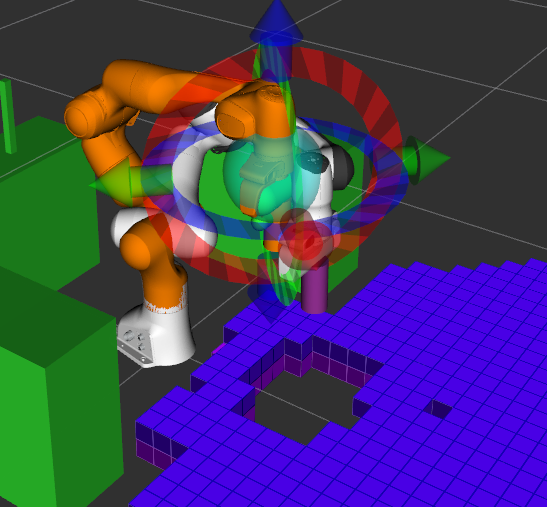
\includegraphics[width=6cm]{images/Q2/grasp1.png}
    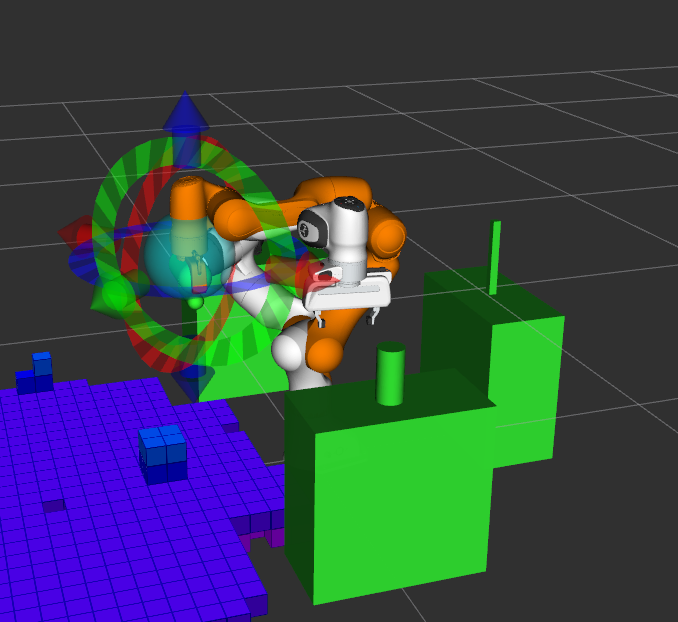
\includegraphics[width=6cm]{images/Q2/grasp2.png}
    \caption{Grasping and placing onto table1 without constraint}
    \label{fig:q2}
\end{figure}
As shown in the figure \ref{fig:q2}, upon pressing ``1", the robot automatically detects the robot at the ground location and moves the robot from the ground location to table1.
\section{Question 3}
This question has posed extra constraints to the pick and place of the object, e.g. the tables and the hindering object (stick) that occupies table 2 at the beginning. Hence we need to use the information published into \texttt{bumper1\_pub}, \texttt{bumper2\_pub} and \texttt{bumper3\_pub} to detect whether the designated table to move the cylinder to is empty. Also, even if the bumper sensor detects that the designated table is occupied, we need to distinguish whether the occupant is cylinder (in which case nothing needs to be done) or the obstruction objects (in which case the object should be moved away to other free tables). \\

In this case, we defined various local variables together with the latest pose information of the cylinder to help the robot decide what to do automatically. Firstly, we check whether the designated table to move to is occupied by checking the information published by the bumper sensors. If the designated table is occupied, we then check whether the occupant is cylinder by checking the latest published pose of the cylinder from \texttt{ROS} topic \texttt{cylinder\_pose}. If the x and y coordinates of the latest cylinder pose match the x and y coordinates of the designated table, we don't need to do anything; else, we need to move the stick object to other free table. \\

Locally, we created a variable \texttt{isCylinder} to indicate whether the current object to be picked and placed is cylinder or not, because the grasping pose changes accordingly. We also defined \texttt{fromTable} and \texttt{toTable} to notify the robot which is the table to pick from and to place the object onto. If the \texttt{toTable} is occupied based on the bumper sensor data, the robot then checks for the occupant identity as described above before moving the cylinder. \\

The work flow for pressing either 1, 2, or 3 are the same. However, the tables and bumpers that we are checking are different subject to the destination table. Below shows the case when we want to move the cylinder to table1:

\begin{lstlisting}[language=C++,
                   directivestyle={\color{black}}
                   emph={int,char,double,float,unsigned},
                   emphstyle={\color{blue}}
                  ]
  if (ch == '1')
  {
    std::string fromTable = "";
    std::string toTable   = "";
    // Check table 1 if there is an object via bumper
    if (cw3_obj.bumper1HasObject)
    {
      if (cw3_obj.objPosX == 0.0 && cw3_obj.objPosY == 0.5)
      {
        // Cylinder already on table one, do nothing.
        ROS_INFO("Cylinder already on table 1");
      }
      else 
      {
        // Stick object on table one, move it to any empty table.
        fromTable = "table1";
        if (!cw3_obj.bumper2HasObject)
        {
          toTable = "table2";
        }
        else if (!cw3_obj.bumper3HasObject)
        {
          toTable = "table3";
        }

        // Move stick
        bool isCylinder = false;
        cw3_obj.pick(move_group, fromTable, isCylinder);
        cw3_obj.place(move_group, toTable, isCylinder);

        // Update sensor value
        if (toTable.compare("table2") == 0)
        {
          cw3_obj.bumper2HasObject = true;
        }
        else if (toTable.compare("table3") == 0)
        {
          cw3_obj.bumper3HasObject = true;
        }
        cw3_obj.bumper1HasObject = false;
      }
    }
    
    if (!cw3_obj.bumper1HasObject)
    {
      // Now find the location of the cylinder
      if (cw3_obj.objPosX == -0.5 && cw3_obj.objPosY == 0.0)
      {
        fromTable = "table2";
      }
      else if (cw3_obj.objPosX == 0.0 && cw3_obj.objPosY == -0.5)
      {
        fromTable = "table3";
      }
      else
      {
        fromTable = "";
      }
      toTable = "table1";

      // Move cylinder
      bool isCylinder = true;
      cw3_obj.pick(move_group, fromTable, isCylinder);
      cw3_obj.place(move_group, toTable, isCylinder);
      cw3_obj.updateCylinderPose(cylinder_pose_pub, toTable);
      cw3_obj.bumper1HasObject = true;

      // Update bumper
      if (fromTable.compare("table2") == 0)
      {
        cw3_obj.bumper2HasObject = false;
      }
      else if (fromTable.compare("table3") == 0)
      {
        cw3_obj.bumper3HasObject = false;
      }
    }
  }
\end{lstlisting}
For full section of the code please refer to the code in \texttt{test\_cw3.cpp}.

\begin{figure}[H]
    \centering
    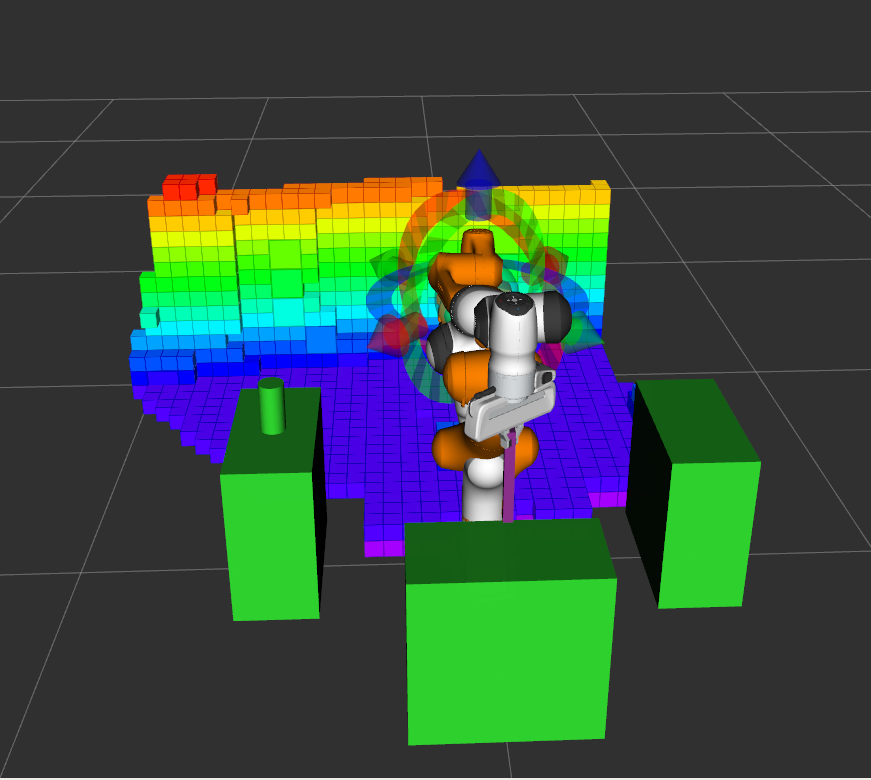
\includegraphics[width=5cm, height=5cm]{images/Q3/2_pickStick.png}
    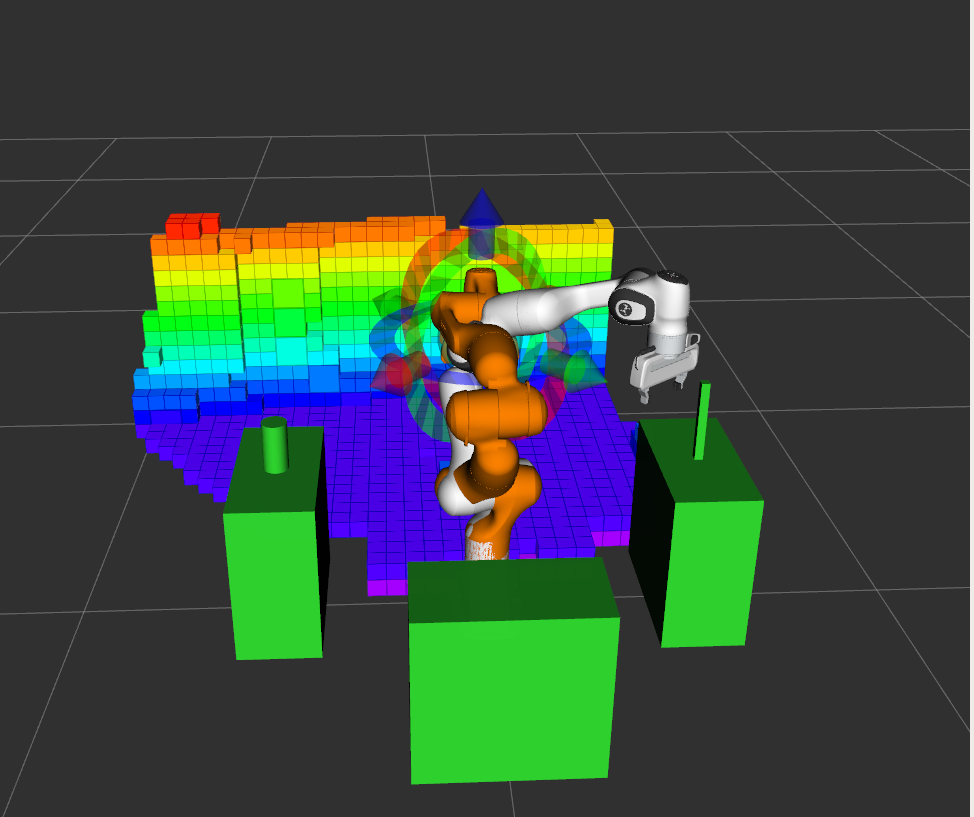
\includegraphics[width=5cm, height=5cm]{images/Q3/2_placeStick.png}\\
    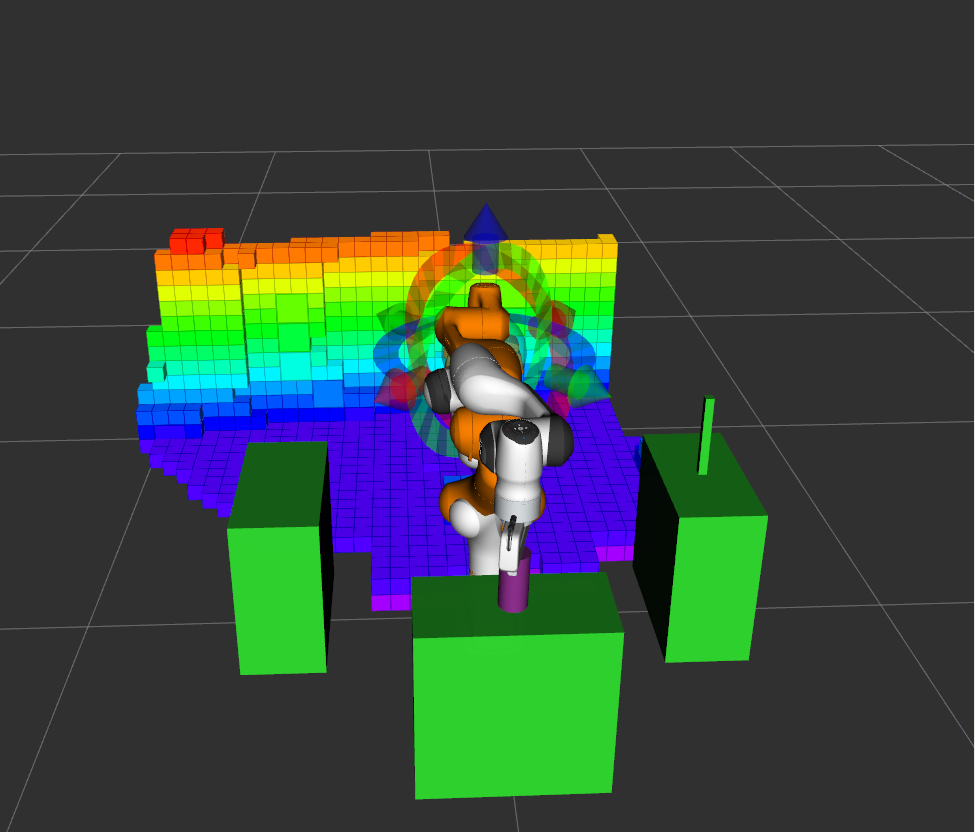
\includegraphics[width=5cm, height=5cm]{images/Q3/2_pickCylinder.png}
    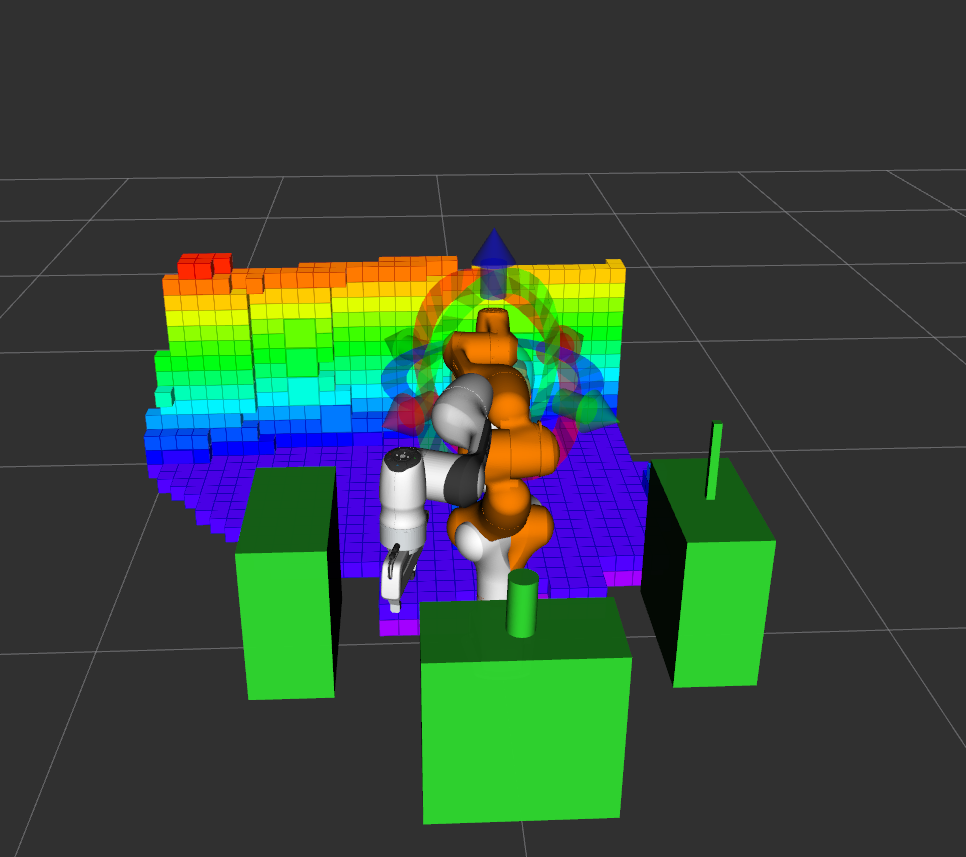
\includegraphics[width=5cm, height=5cm]{images/Q3/2_placeCylinder.png}
    \caption{Robot picks stick from table 2 and places stick onto table 3, then pick the cylinder from table 1 and places it on table 2}
    \label{fig:2_pickPlace}
\end{figure}

The I/O implementation is done in \texttt{test\_cw3.cpp} for the key pressing. As shown in figure \ref{fig:2_pickPlace}, when pressing "2", the robot moves the stick object from table 2 to the empty table 3, before moving the cylinder from table 1 to table 2.\\

\begin{figure}[H]
    \centering
    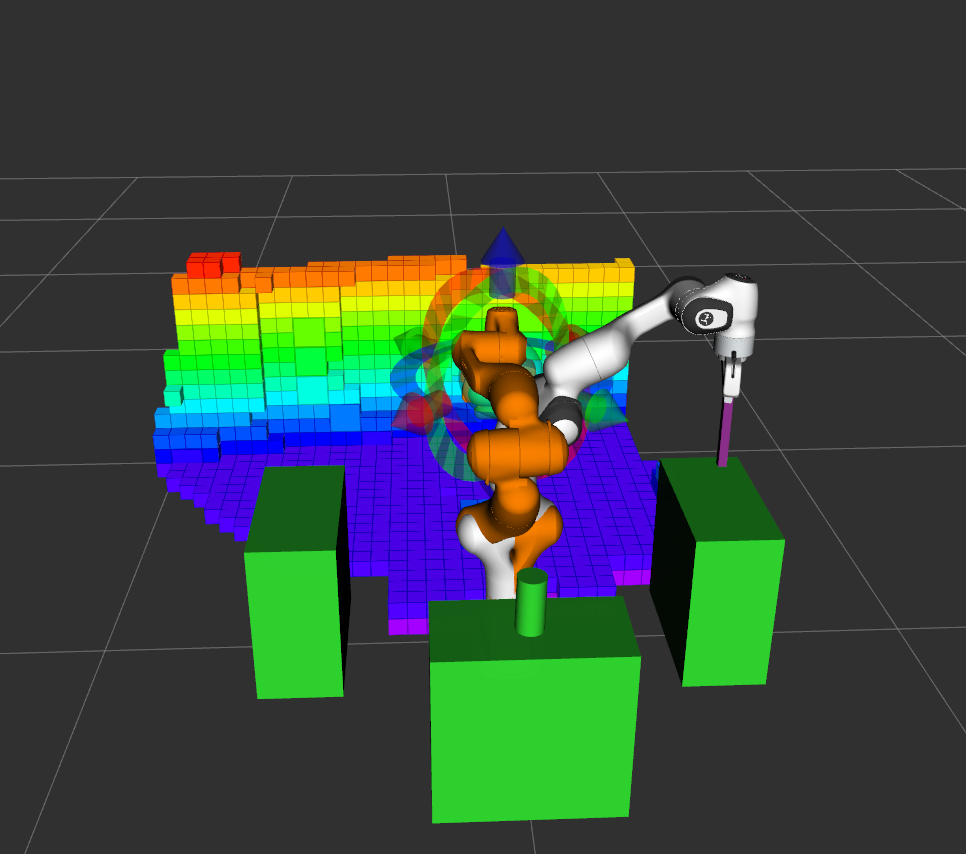
\includegraphics[width=5cm, height=5cm]{images/Q3/3_pickStick.png}
    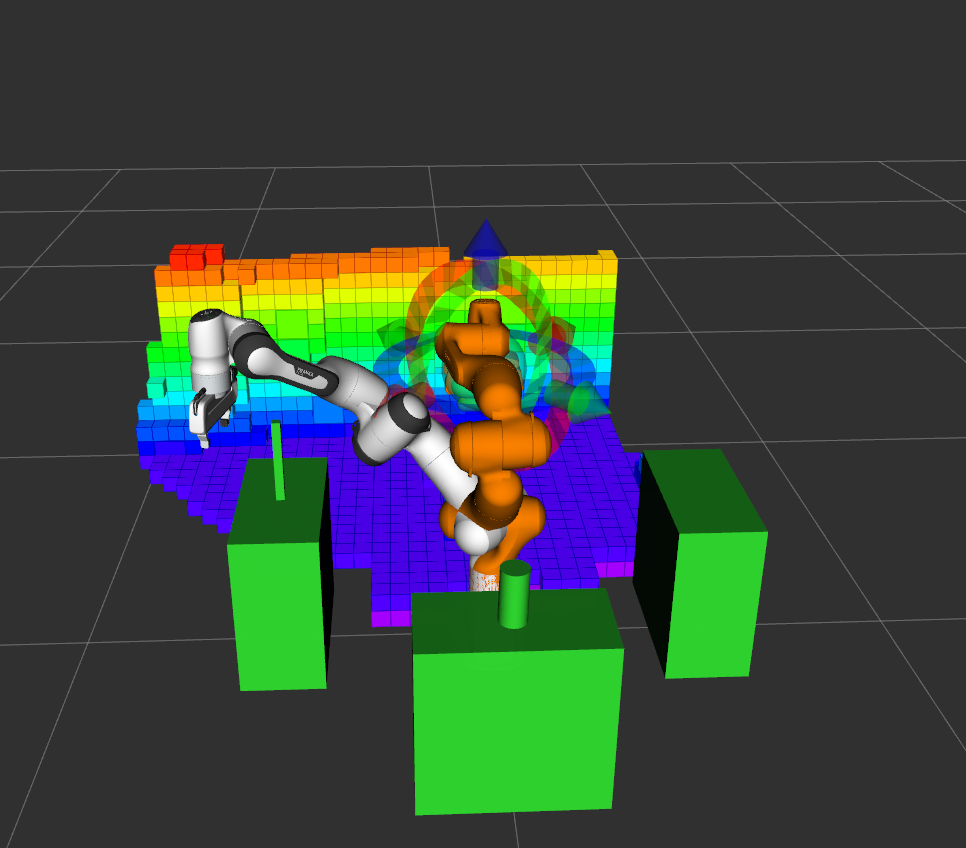
\includegraphics[width=5cm, height=5cm]{images/Q3/3_placeStick.png}\\
    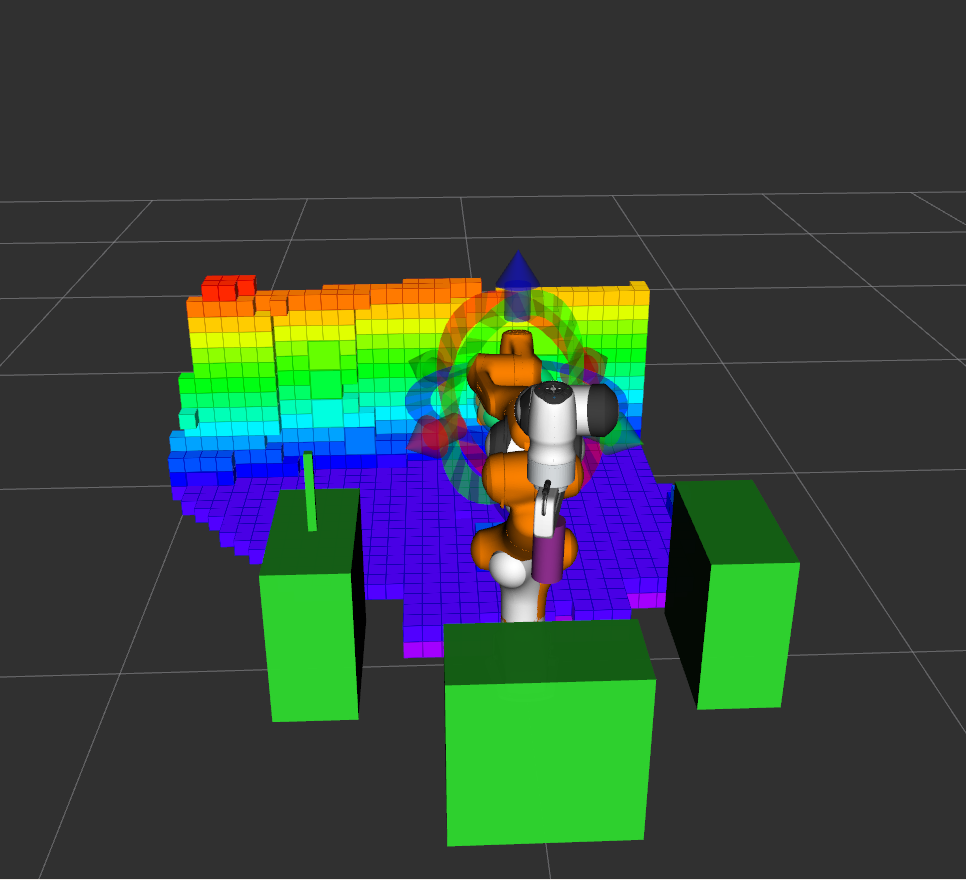
\includegraphics[width=5cm, height=5cm]{images/Q3/3_pickCylinder.png}
    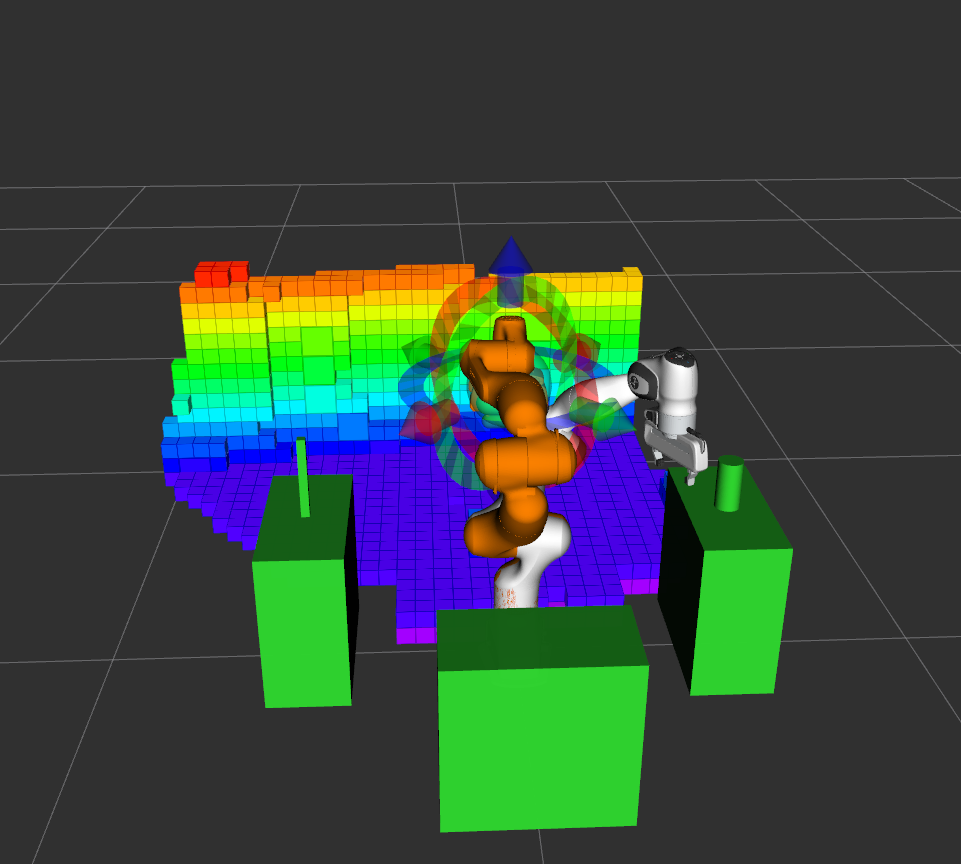
\includegraphics[width=5cm, height=5cm]{images/Q3/3_placeCylinder.png}
    \caption{Robot picks stick from table 3 and places stick onto table 1, then pick cylinder from table 2 and places it on table 3}
    \label{fig:3_pickPlace}
\end{figure}

Similarly, as shown in figure  \ref{fig:3_pickPlace}, when pressing ``3", the robot moves the stick object from  table 3 to the empty table 1, before moving the cylinder from table 2 to table 3.\\
 
During the development, we have discovered that we also need different parameters for pre-grasp approach and post-grasp retreat. We have tried different numbers and found the following worked. These are implemented in the function \texttt{void CW3::place()} at \texttt{cw3.cpp}:

\begin{lstlisting}[language=C++,
                   directivestyle={\color{black}}
                   emph={int,char,double,float,unsigned},
                   emphstyle={\color{blue}}
                  ]

  if(isCylinder)
  {
    // Approach
    place_location[0].pre_place_approach.min_distance     = 0.05;
    place_location[0].pre_place_approach.desired_distance = 0.15;

    // Retreat
    place_location[0].post_place_retreat.min_distance     = 0.1;
    place_location[0].post_place_retreat.desired_distance = 0.25;
  }
  else
  {
    // Approach
    place_location[0].pre_place_approach.min_distance     = 0.05;
    place_location[0].pre_place_approach.desired_distance = 0.35;

    // Retreat
    place_location[0].post_place_retreat.min_distance     = 0.05;
    place_location[0].post_place_retreat.desired_distance = 0.55;
  }
\end{lstlisting}
\bibliographystyle{IEEEtran}
\bibliography{references}
\end{document}

